\documentclass{fisatprojectfinal}
\title{Real Time Crowd Detection}
\team{Emmanuel Jojy}
\author{Emmanuel Jojy}
\regno{FIT19CS049}
\linespread{1.5}
\begin{document}
\maketitle
\makecert

\newpage
\renewcommand\abstractname{Declaration}
\thispagestyle{plain}
\begin{abstract}
\vspace{5cm}
I hereby declare that the project report {\bf{\title}}, submitted for partial fulfillment of the requirements for the award of degree of Bachelor of Technology of the APJ Abdul Kalam Technological University, Kerala is a bonafide work done by us under supervision of Mr. Pankaj Kumar G, Assistant Professor, Department of Computer Science and Engineering. \par
This submission represents my ideas in our my words and where ideas or words of others have been included, we have adequately and accurately cited and referenced the original sources.\par 
I also declare that I have adhered to ethics of academic honesty and integrity and have not misrepresented or fabricated any data or idea or fact or source in my submission. I understand that any violation of the above will be a cause for disciplinary action by the institute and/or the University and can also evoke penal action from the sources which have thus not been properly cited or from whom proper permission has not been obtained. This report has not been previously formed the basis for the award of any degree, diploma or similar title of any other University.
\vspace{1cm}
\begin{flushright}
Emmanuel Jojy
\end{flushright}
Mookanoor\\ 
14/09/2022


\end{abstract}

%
\newpage
\renewcommand\abstractname{Contribution by Author}
\thispagestyle{plain}
\begin{abstract}
\vspace{5cm}
Devised the idea of a two stage model for easy and efficient crowd detection. The YOLOv4 framework was integrated with the sate-of-the-art tracking algorithm DeepSORT. The output of the former was normalized and then fed into a clustering algorithm. Finally based on clusters generated the crowd bounding boxes were also drawn.  
\vspace{1cm}
\begin{flushright}
Emmanuel Jojy
\end{flushright}
\end{abstract}
%
\newpage
\renewcommand\abstractname{ACKNOWLEDGEMENT}
\thispagestyle{plain}
\begin{abstract}
\vspace{5cm}
\par I take this opportunity to express my deepest sense of gratitude and sincere thanks to everyone who helped us to complete this work successfully. I express my sincere thanks to \textbf{Dr. Jyothish K John}, Head of Department, Department of Computer Science and Engineering, Federal Institute of Science and Technology for providing us with all the necessary facilities and support.

I would like to express my sincere gratitude to Project Coordinators \textbf{Ms. Chethna Joy} and \textbf{Ms. Remya R} for their support and co-operation.

I would like to place on record my sincere gratitude to our project guide \textbf{Mr. Pankaj Kumar G}, for the guidance and mentorship throughout this work. Had it not been for his guidance and support this project would never be a reality. 

Finally I thank my family, and friends who contributed to the successful fulfilment of this seminar work.
\vspace{1cm}
\begin{flushright}
Emmanuel Jojy
\end{flushright}
\end{abstract}

\newpage
\pagenumbering{roman}
\setcounter{page}{1}
\newgeometry{top=4cm,bottom=0.1cm}
\thispagestyle{plain}
\renewcommand\abstractname{ABSTRACT}
\begin{abstract}
\vspace{5cm}

Crowd is a unique group of individual or something involves community or society. The phenomena of the crowd are very familiar in a variety of research discipline such as sociology, civil and physic. Nowadays, it becomes the most active-oriented research and trendy topic in computer vision. Traditionally, three processing steps involve in crowd analysis, and these include pre-processing, object detection and event/behavior recognition. Here, an efficient framework with two phases for preliminary crowd analysis is developed, the detection and clustering. For detection the state of the art YOLO model is used in combination with DeepSORT.  DBSCAN is used in the second phase as the clustering variant.
\end{abstract}




\newpage

\restoregeometry
\tableofcontents
\thispagestyle{plain}
\newpage

\cleardoublepage
\addcontentsline{toc}{chapter}{\listfigurename}
\listoffigures
\newpage

\cleardoublepage
\addcontentsline{toc}{chapter}{\listtablename}
\listoftables
\newpage


\chapter{Introduction}
\pagenumbering{arabic}
\setcounter{page}{1}
\renewcommand{\baselinestretch}{1.50}
\section{Overview}
\par Video surveillance is the facility to observe and analyze any particular site for identifying suspicious activity with respect to safety and security purposes. Video surveillance system came into existence for security and crime control in the society. Currently, video cameras are used for such kind of surveillance and they can be deployed in several places easily such as companies, railway stations, shopping centers, bank offices and ATM machines etc. Some decades ago, video surveillance system were not so much prevalent as of today. Various changes in this period have resulted in deployment and growth of video surveillance system. 
\begin{figure}[h!]
\begin{center}
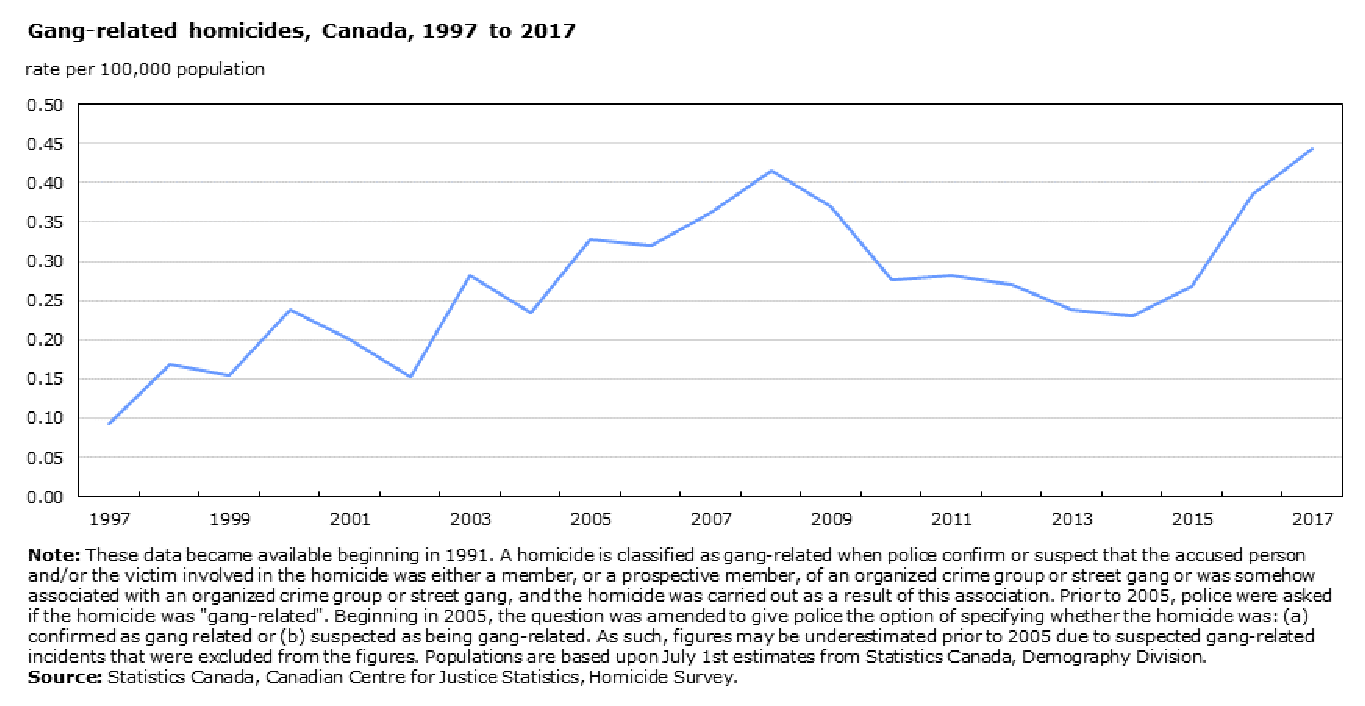
\includegraphics[scale=.6]{img_homiciderate.eps}
\caption{Gang-related homicides statistics}
\end{center}
\end{figure}
Last years have known a significant increase of crime and terrorism. Video-surveillance has become a crucial tool for preventing violence and crimes, especially in crowded places and events. The number of video cameras installed in both, public and private places, multiplied in the last years. Human social dysfunction is changing and their approach to security is becoming more sensible. In present time, everyone is getting familiar with technological platform to handle different security tasks. CCTV usage is getting more popular with the price affordability and less effort for their setup. On the other hand, technology advances allowed an unprecedented improvement in video quality but at the cost of higher computational requirements.

\begin{table}[h!]
\begin{center}
	\caption{CCTV count by cities} 
\vspace{0.25in}
\begin{tabular}{|c|c|c|c|}
	
\hline Rank & City & Country & Count ( per sq. mile )  \\ 
\hline 1 & Delhi & India & 1826\\ 
\hline 2 & London & United Kingdom & 1138.48\\
\hline 3 & Chennai & India & 609.92\\ 
\hline 4 & Shenzhen & China & 520.08\\ 
\hline 5 & Wuxi & China & 472.66\\ 
\hline 6 & Qingdao & China & 415.80\\
\hline 7 & Shanghai & China & 415.80\\ 
\hline 8 & Singapore & Singapore & 387.56\\ 
\hline 9 & Changsha & China & 353.85\\ 
\hline 10 & Wuhan & China & 339.01\\ 
\hline 11 & Seoul & South Korea & 331.94\\
\hline 12 & Moscow & Russia & 210.01\\ 
\hline 13 & New York & United States & 193.72\\
\hline 
\end{tabular}
%\caption{CCTV count by cities} 
\end{center}
\end{table}


\par Formally, Monitoring system consists of large number of cameras that helps to monitor different sites. It is used to detect any noticeable and unwanted or illegal activity, so as to immediately respond to the situation with very short delay. These surveillance system are fruitless to provide security, until inadequate capacity of trained people with their high attention competence are fulfilled for watching the flicks. Sometimes, searching specific activity from the large amount of recorded videos files seems very difficult and time consuming process for examining the occurred event. Hence, it requires computer vision system.
\begin{figure}[h!]
\begin{center}
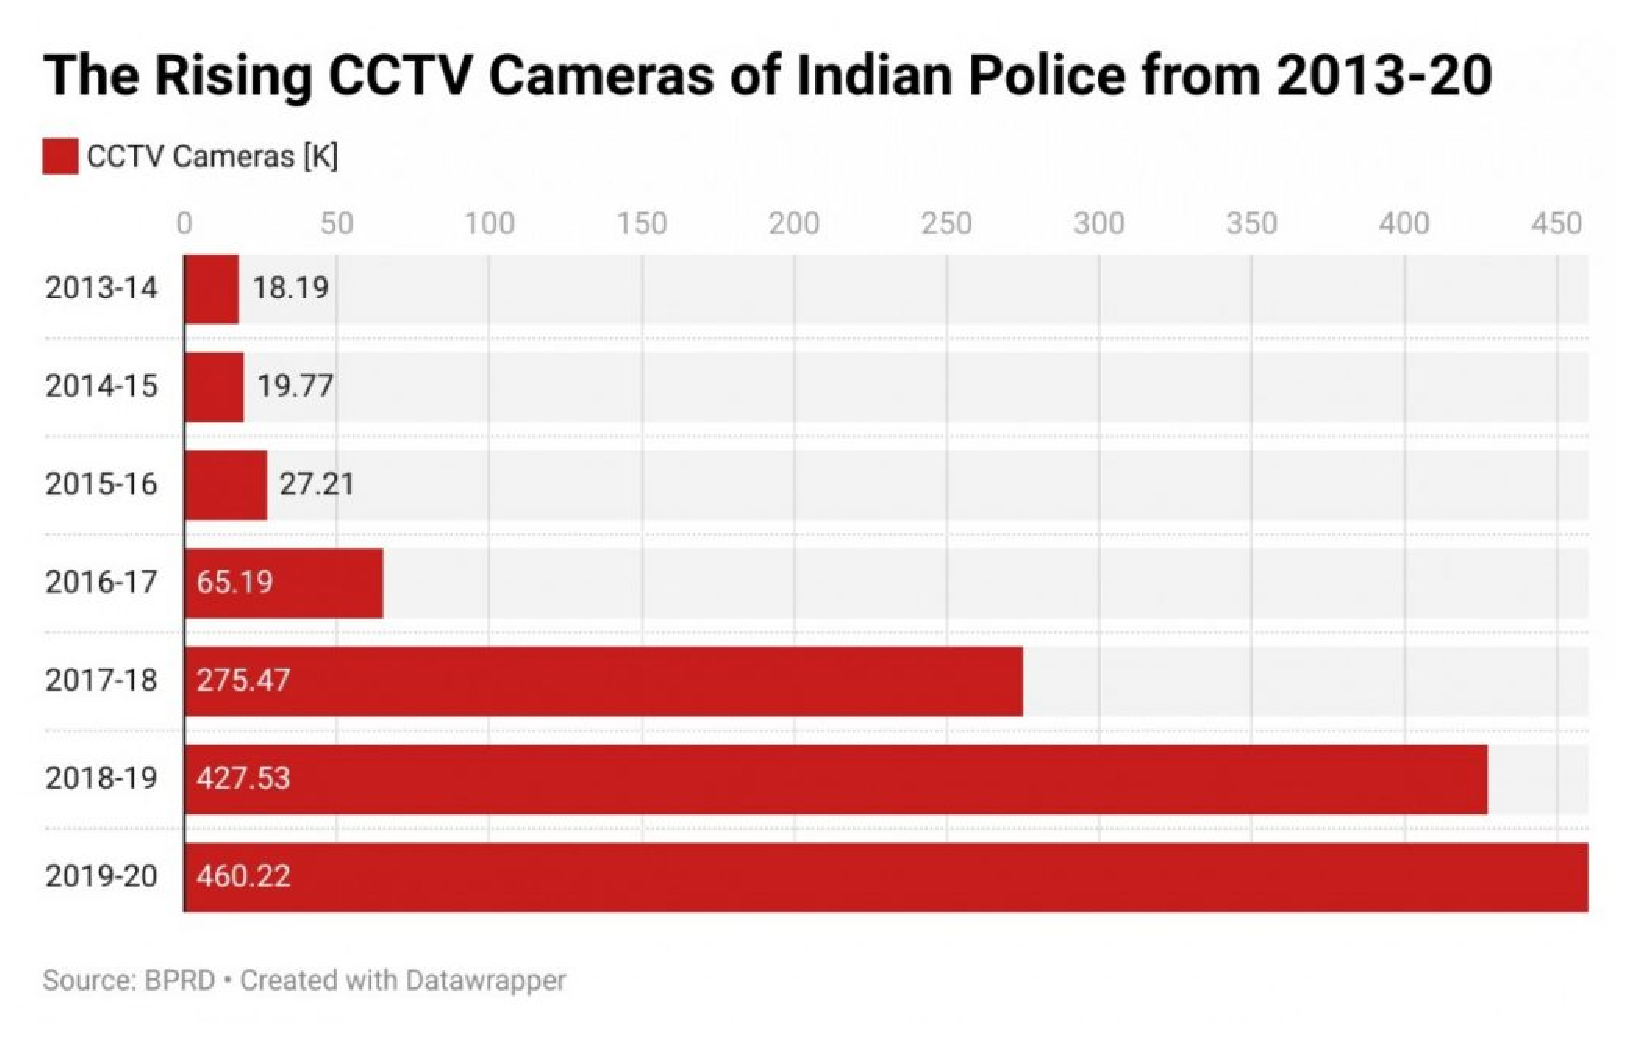
\includegraphics[scale=.45]{img_cctvtrend.eps}
\caption{Indian Police, CCTV statistics}
\end{center}
\end{figure}
\par Automatic video-surveillance, including crowd behaviour analysis, is increasingly attracting much attention. This area aims to understand how individuals behave when they are part of a large group, and extract meaningful information from videos in which crowds of people are present. For example, the automatic analysis of the motion flow of pedestrians when accessing a crowded pilgrimage site, or monitoring the behaviour of large amounts of fans in a sport stadium is crucial in order to detect dangerous situations previous to a catastrophe.
\par I hereby propose a two stage solution for first phase crowd detection. The first stage is a basic detection system using YOLOv4, capable of detecting individuals coupled with DeepSORT for enhanced feature based tracking. The second stage uses a clustering algorithm to cluster individuals based on spatial data from former and group them into crowd. The clustering algorithm employed is the standard DBSCAN algorithm. 

\section{Problem Statement}
With the rapid urbanization and development of big cities and towns, the graph of crimes specifically is also on the increase,  which is a matter of great concern and alarm to all of us. To cope with this problem, surveillance systems are being widely used all around. But monitoring such humongous data, in our case keeping track of crowd activity, round the clock manually is inefficient and prone to errors. To cope with this automated real time video surveillance with crowd detection is a must. In this project I aim to implement Real Time Crowd Detection. 

\section{Objective}

The project aims to implement a lightweight real time crowd detection system using a two stage system. The target application being CCTV cameras and other related resource constrained devices, the model developed must be efficient, real time and lightweight. 

\chapter{Related works}

There is a need for establishing a common ground for the analysis and characterisation of crowd behaviour. The first definition to be remarked is about what should be considered a crowd. A proper way to define the concept of crowd is through its differentiation from the concept of group:

\begin{itemize}
  \item Group: It consists on a collection of people that can range from a
size of two persons to hundreds, in mutual presence at a given moment, who are having some form of social interaction. Its members are close to each other, with a similar speed and with a similar direction of motion.
  \item Crowd (or mass): A crowd is a unique large group of individuals sharing a common physical location. It is usually formed when people with the same goal become one single entity, losing their individuality and adopting the behaviour of the crowd entity. Complex crowd behaviours may result from repeated simple interactions among its constituent individuals, i.e., individuals locally coordinate their behaviours with their neighbours, and then the crowd is self-organised into collective motions without external control
\end{itemize}

Therefore, the definition of these two terms can be clarified by using two different features: the density of individuals, which is higher in crowds; and the relationships and interactions between the individuals, which tend to be higher in groups. A group is usually formed by less people, with a stronger relation and cohesion. A crowd typically refers to a much larger collection of subjects, whose relationships are less stronger, and with an organisation that emerges from the individual interaction between agents.

Once the concept of crowd is properly defined, delimiting the scope of the area becomes the next challenge. There are many different suitable interpretations for the task of crowd behaviour analysis. In general terms, the main goal in the area is to be able to understand how a concentration of individuals behaves, using information retrieved mainly from video sources. 

However, there are a lot of different aspects in the behaviour of a crowd we can be interested in. For example, the number of subjects on a certain location and how this number varies in a period of time can be useful to prevent dangerous stampedes of pedestrians. Also, the understanding of the predominant motion directions in a moving crowd (e.g. when accessing a sport stadium) may be useful to detect the persons whose movement differs from the main flows and identify their reasons. A few major crowd analysis categorization are as follows:

\begin{itemize}
  \item Crowd detection and tracking. It covers the works whose task is to follow the trajectory of pedestrians in a video. Multiple Object Tracking (MOT), when focused on pedestrians, belongs to this subarea. It also covers the tracking of crowds, i.e., the estimation of the flow of a large group of people moving.
  \item Crowd counting. The works whose aim is to estimate the number of individuals present in a video are included in this category.
  \item Crowd behaviour classification. This task involves the identification and classification of behaviours usually known a priori.
  \item Crowd anomaly detection. In this case, the task is to identify abnormal behaviours in a crowd, not known a priori. It is an anomaly detection approach to the problem
\end{itemize}

This categorisation includes the main sub-tasks in the topic, but places all of them at the same level. However, it is clear that there is a hierarchical relation among the four mentioned tasks, and some of them can be performed as consecutive steps of a pipeline. For instance, the crowd counting stage is often performed after the detection and tracking of individuals. The output of crowd counting may also be used as an input feature for detecting abnormal behaviour, such as congestion. In the next section, we propose a categorisation that overcomes the absence of hierarchy of the previous works, while keeping their contributions as different parts of a pipeline.

Few works have tried to organise the advances in the field by categorising the problems/tasks that it constitutes, even though such categorisations could be very useful for comparing related works that address the same task. 


\chapter{Design}
\section{Introduction}
An illustration of our proposed architecture for crowd behavior recognition is shown in Fig. 3.1. It has two main stages: Person detection and tracking, and clustering. 

\begin{figure}[h!]
\begin{center}
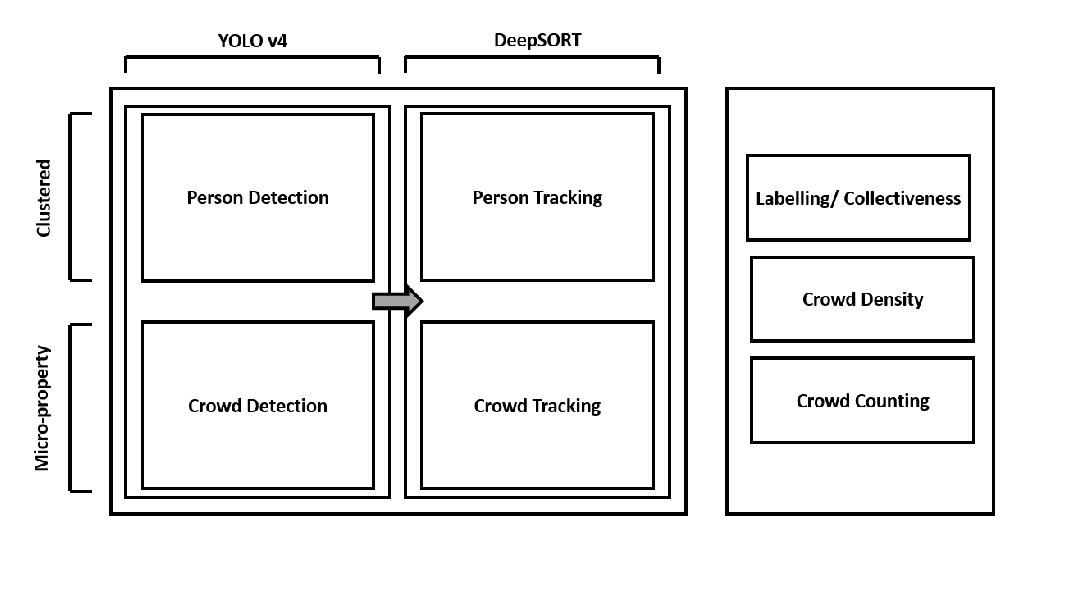
\includegraphics[scale=0.95]{img_pipelinebasic.eps}
\caption{Proposed project stages}
\end{center}
\end{figure}

The former is implemented using a combination of YOLOv4 and DeepSORT, while the latter uses standard clustering technique DBSCAN. Since the model works real time the input to the model is live image, frame by frame. The frame rate is dependent largely on first stage.  


\section{Modules}
\subsection{YOLOv4}
The majority of CNN-based object detectors are largely applicable only for recommendation systems. For example, searching for free parking spaces via urban video cameras is executed by slow accurate models, whereas car collision warning is related to fast inaccurate models. Improving the real-time object detector accuracy enables using them not only for hint generating recommendation systems, but also for stand-alone process management and human input reduction. Real-time object detector operation on conventional Graphics Processing Units (GPU) allows their mass usage at an affordable price. 

\begin{figure}[h!]
\begin{center}
\includegraphics[scale=.75]{img_yolovsothers.eps}
\caption{Comparison of YOLOv4 and other state-of-the-art detectors}
\end{center}
\end{figure}

The most accurate modern neural networks do not operate in real time and require large number of GPUs for training with a large mini-batch-size. Whereas the YOLOv4 model offers a state-of-the-art detector which is faster and more accurate than all available alternative detectors without compromising AP and FPS. Since it allows for a high frame rate it is extremely suitable for Real Time Applications.

Citing all these advantages YOLOv4 was chosen for detection part. For person detection  the MS COCO dataset was made use. The MS COCO dataset consist of a total of 80 classes including person class.

\subsection{DeepSORT}
DeepSORT or SORT with a Deep Association Metric is an extension to SORT (Simple Online and Realtime Tracking). It is a pragmatic approach to multiple object tracking with a focus on simple, effective algorithms. 

\begin{figure}[h!]
\begin{center}
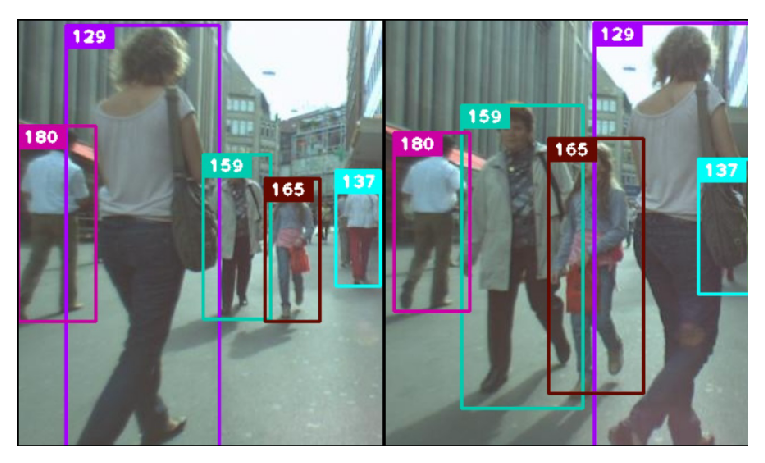
\includegraphics[scale=.8]{img_deepsort.eps}
\caption{DeepSORT on the MOT Challenge Dataset}
\end{center}
\end{figure}

DeepSORT uses a better association metric that combines both motion and appearance descriptors. DeepSORT can be defined as the tracking algorithm which tracks objects not only based on the velocity and motion of the object but also the appearance of the object. SORT also shows high AP over long periods of occlusion which is common in any high dense crowded environment. In contrast to SORT identity switches have been drastically reduced in DeepSORT. 

With DeepSORT we assign a unique identifier to the tracked object, in our case person. Based on the generated identifier a persons inclusiveness or exclusiveness in a group is determined. DeepSORT is a strong competitor to other online trackering frameworks such as SORT and POI.

A frame log from the project after running YOLOv4 and DeepSORT over a sample: 
\begin{verbatim}
    Frame Data
    {0: [742, 220, 886, 405]}
    Frame data Frame #: 14
    Tracker ID: 01, Class: person,  BBox: (192, 843, 298, 1080)
    Tracker ID: 02, Class: person,  BBox: (743, 219, 811, 400)
    Tracker ID: 03, Class: person,  BBox: (1604, 640, 1724, 910)
    Tracker ID: 04, Class: person,  BBox: (895, 71, 957, 222)
    Tracker ID: 05, Class: person,  BBox: (829, 231, 888, 404)
    Tracker ID: 06, Class: person,  BBox: (817, 417, 947, 650)
    Tracker ID: 07, Class: person,  BBox: (1647, 107, 1712, 262)
    Tracker ID: 09, Class: person,  BBox: (1466, 29, 1546, 177)
    Tracker ID: 11, Class: person,  BBox: (1813, 172, 1884, 338)
    Tracker ID: 12, Class: person,  BBox: (605, 959, 855, 1079)
    Tracker ID: 13, Class: person,  BBox: (1146, 0, 1188, 76)
    Tracker ID: 14, Class: person,  BBox: (1323, 0, 1355, 38)
    Tracker ID: 16, Class: person,  BBox: (992, 0, 1055, 122)
    Tracker ID: 17, Class: person,  BBox: (317, 219, 394, 409)
    FPS: 14.88
\end{verbatim}
Note that for the frame, bounding box coordinates (BBox) are generated by YOLOv4 whereas Tracker ID's are generated correspondingly by DeepSORT. The frame data would be the input to the next stage.

\subsection{DBSCAN}
DBSCAN or Density-based spatial clustering of applications with noise (DBSCAN) is a data clustering algorithm proposed in 1996. It is a density-based clustering non-parametric algorithm: given a set of points in some space, it groups together points that are closely packed together (points with many nearby neighbors), marking as outliers points that lie alone in low-density regions (whose nearest neighbors are too far away). DBSCAN is one of the most common clustering algorithms and also most cited in scientific literature.

\begin{figure}[h!]
\begin{center}
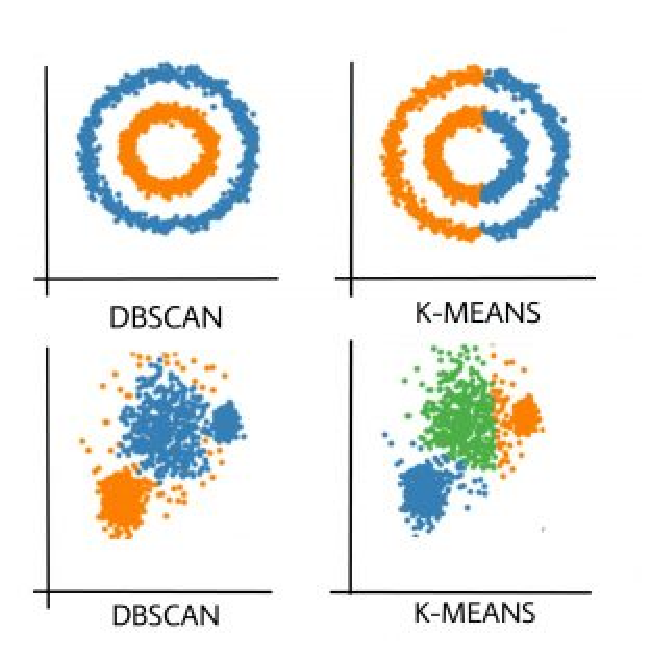
\includegraphics[scale=.75]{img_dbscan.eps}
\caption{Comparison of DBSCAN and K-MEANS clustering algorithm}
\end{center}
\end{figure}

DBSCAN was chosen as the clustering algorithm specifically because of the following factors:

\begin{itemize}
  \item DBSCAN does not require one to specify the number of clusters in the data, as opposed to k-means. Surveillance footage is highly dynamic and since number of individual crowd(s) cannot be estimated beforehand DBSCAN was chosen over other algorithms.
  \item DBSCAN has a notion of noise, and is robust to outliers. Unlike K-MEANS and other similar clustering algorithms, DBSCAN discards noise, which our application is highly prone to. 
  \item DBSCAN requires just two parameters and is mostly insensitive to the ordering of the points in the database. The MinPts can be used to define the threshold, indicating number of minimum people in a group, and can be easily modified based on the environment.  
  \item DBSCAN can find arbitrarily-shaped clusters. It can even find a cluster completely surrounded by (but not connected to) a different cluster. This happens usually in our case when people form a shape similar to that of concentric circles.
\end{itemize}

\section{Dataset}
\subsection{MS COCO Dataset}
MS COCO (Microsoft Common Objects in Context) is a large-scale image dataset containing 328,000 images of everyday objects and humans. The dataset contains annotations you can use to train machine learning models to recognize, label, and describe objects. 

MS COCO provides the following types of annotations:

\begin{itemize}
    \item detection—coordinates of bounding boxes and full segmentation masks for 80 categories of objects.
    \item Object detection—coordinates of bounding boxes and full segmentation masks for 80 categories of objects
    \item Captioning—natural language descriptions of each image.
    \item Keypoints—the dataset has more than 200,000 images containing over 250,000 humans, labeled with keypoints such as right eye, nose, left hip.
    \item “Stuff image” segmentation—pixel maps of 91 categories of “stuff”—amorphous background regions like walls, sky, or grass.
    \item Panoptic—full scene segmentation, indicating objects in the image according to 80 categories of “things” (cat, pen, fridge, etc.) and 91 “stuff” categories (road, sky, water, etc.).
    \item Dense pose—the dataset has more than 39,000 images containing over 56,000 humans, with every labeled person annotated with an instance id and a mapping between pixels representing that person’s body and a template 3D model.
\end{itemize}

\section{Conclusion}
Once first stage processing, YOLOv4 and DeepSORT pipeline, was complete, the result was transferred to stage two, DBSCAN clustering. These steps for invoked for each frame consecutively making it real-time. The effective FPS initally for YOLOv4 dropped by some extend due to the incorporation of DeepSORT tracking. 

The final output would be the same frame but with bounding boxes over the crowd. OpenCV was used for this purpose.

\chapter{Results}

The model was tested against the Oxford Town Centre Dataset and Wildtrack Seven Camera Dataset and the output are as follows:

\newpage
\thispagestyle{plain} % empty
\mbox{}

\chapter{Conclusion}

A simple two stage model for Real Time crowd detection was implemented and showed promising results. Hopefully the model could be used in practical scenarios as in detection of an instantaneous crowd in a locality or for even town planning. This model could be used as basis for other related CCTV surveillance applications, which can be built over the same, such as crowd anomaly detection and crowd behaviour detection. The model if employed using tiny-YOLOv4 would be a suitable embedded software for resource constrained devices.


\begin{thebibliography}{1}
\bibitem{source} Rezaei, F., Yazdi, M. Real-time crowd behavior recognition in surveillance videos based on deep learning methods. J Real-Time Image Proc 18, 1669–1679 (2021). \url{https://doi.org/10.1007/s11554-021-01116-9}

\bibitem{taxonomy} Francisco Luque Sánchez, Isabelle Hupont, Siham Tabik, Francisco Herrera, "Revisiting crowd behaviour analysis through deep learning: Taxonomy, anomaly detection, crowd emotions, datasets, opportunities and prospects," Information Fusion, Volume 64, 2020, pg 318-335, \url{https://doi.org/10.1016/j.inffus.2020.07.008.}.

\bibitem{yolov4} Bochkovskiy, Alexey and Wang, Chien-Yao and Liao, Hong-Yuan Mark, "YOLOv4: Optimal Speed and Accuracy of Object Detection", \url{https://arxiv.org/abs/2004.10934}.

\bibitem{deepsort} Nicolai Wojke, Alex Bewley, Dietrich Paulus, "Simple Online and Realtime Tracking with a Deep Association Metric", \url{https://arxiv.org/abs/1703.07402}.

\bibitem{DBSCAN} Martin Ester, Hans-Peter Kriegel, Jiirg Sander, Xiaowei Xu, "A Density-Based Algorithm for Discovering Clusters
in Large Spatial Databaseswith Noise", \url{https://www.aaai.org/Papers/KDD/1996/KDD96-037.pdf}.
\end{thebibliography}

\begin{appendices}

\paragraph{1. Basic Grouping}
\begin{verbatim}
    import re
    from logic.model import Person
    from logic.util import cluster, map_label, left_most, right_most
    
    frames = {}
    cv_input = {}
    def generate_group(frame_id, clusters):
        # Single Frame Activation Code
        global cv_input
        cv_input = {}
        for cluster_id, people in clusters.items():
            tl_coordinates = [person.box.tl for person in people]
            br_coordinates = [person.box.br for person in people]
            lm = left_most(tl_coordinates)
            rm = right_most(br_coordinates)
            cv_input[cluster_id] = [lm.x, lm.y, rm.x, rm.y]
            
    def analyze_frame(frame_id, people):
        coordinate_list = [list(person.getCentre()) for person in people]
        cluster_map = map_label(people, cluster(coordinate_list))
        clusters = {}
        for point in cluster_map:
            person, cluster_id = point[0], point[1]
            if cluster_id != -1:
                if cluster_id not in clusters:
                    clusters[cluster_id] = [person]
                else:
                    clusters[cluster_id].append(person)
        frames[frame_id] = generate_group(frame_id, clusters)
    
    def analyze_file(frame_data = None):
        global x
        # file = open('out.txt', 'r')
        file = frame_data.split('\n')
        people = []
        frame_id = 0
        print('Frame data', frame_data)
        for line in file:
            if re.search('\AFrame', line):
                # Set new frame_id
                frame_id = int(line[9:].strip())
            elif re.search('\ATracker', line):
                # YOLO Person as Tracker: id
                tracker_id = int(line[11: line.find(',')].strip())
                # Find content in first parenthesis
                coordinates = re.findall(r'\((.*?)\)', line)[1].split(', ')
                # Generate Person 
                p = Person(tracker_id, coordinates)
                people.append(p)
            elif re.search('\AEOF', line) or re.search('\AFPS', line):
                # Frame complete
                if people == []:
                    continue
                analyze_frame(frame_id, people)
        return cv_input
    #from draw import drawBox
    analyze_file()
\end{verbatim}

\paragraph{2. Clustering}
\begin{verbatim}
    """
    Created on Thu Jul 28 13:17:33 2022
    @author: emmij
    """
    import numpy as np
    from sklearn.cluster import DBSCAN
    def cluster(coordinate_list):
        X = np.array(coordinate_list)
        clustering = DBSCAN(eps=100, min_samples=2).fit(X)
        return clustering.labels_
\end{verbatim}
\end{appendices}

\paragraph{3. Subset of actual log file}
The frame data for a subset of the Oxford Town Centre Dataset is attached herewith. The data is to be interpreted as follows:

\begin{table}[h!]
\begin{center}
	\caption{Frame data interpretation} 
\vspace{0.25in}
\begin{tabular}{|c|c|c|c|}
	
\hline Line & Purpose \\ 
\hline 1 & Frame Data Indication\\
\hline 2 & Group and members\\
\hline 3 & Frame Number\\
\hline 4 - & Tracker ID with bounding box coordinates\\
\hline
\end{tabular}
%\caption{Frame data interpretation} 
\end{center}
\end{table}


\begin{verbatim}
    Frame Data
    {0: [1208, 13, 1316, 154]}
    Frame data Frame #: 250
    Tracker ID: 02, Class: person,  BBox: (1208, 13, 1260, 144)
    Tracker ID: 05, Class: person,  BBox: (1274, 22, 1317, 154)
    Tracker ID: 12, Class: person,  BBox: (1248, 349, 1340, 518)
    Tracker ID: 13, Class: person,  BBox: (739, 128, 794, 235)
    Tracker ID: 28, Class: person,  BBox: (1590, 906, 1697, 1080)
    Tracker ID: 30, Class: person,  BBox: (350, 355, 441, 569)
    Tracker ID: 33, Class: person,  BBox: (1413, 0, 1468, 101)
    Tracker ID: 35, Class: person,  BBox: (1420, 857, 1586, 1079)
    Tracker ID: 40, Class: person,  BBox: (29, 378, 109, 586)
    FPS: 12.51
    
    Frame Data
    {0: [1208, 13, 1317, 154]}
    Frame data Frame #: 251
    Tracker ID: 02, Class: person,  BBox: (1209, 12, 1261, 145)
    Tracker ID: 05, Class: person,  BBox: (1275, 22, 1318, 153)
    Tracker ID: 12, Class: person,  BBox: (1248, 347, 1342, 519)
    Tracker ID: 13, Class: person,  BBox: (736, 127, 791, 236)
    Tracker ID: 28, Class: person,  BBox: (1590, 918, 1693, 1079)
    Tracker ID: 30, Class: person,  BBox: (352, 353, 443, 568)
    Tracker ID: 33, Class: person,  BBox: (1410, 0, 1465, 103)
    Tracker ID: 35, Class: person,  BBox: (1423, 853, 1587, 1079)
    Tracker ID: 40, Class: person,  BBox: (36, 375, 115, 580)
    FPS: 14.36
    
    Frame Data
    {0: [1209, 12, 1318, 153]}
    Frame data Frame #: 252
    Tracker ID: 02, Class: person,  BBox: (1210, 9, 1263, 146)
    Tracker ID: 05, Class: person,  BBox: (1277, 21, 1320, 153)
    Tracker ID: 12, Class: person,  BBox: (1249, 346, 1345, 520)
    Tracker ID: 13, Class: person,  BBox: (732, 128, 787, 238)
    Tracker ID: 28, Class: person,  BBox: (1589, 926, 1688, 1079)
    Tracker ID: 30, Class: person,  BBox: (354, 352, 445, 568)
    Tracker ID: 33, Class: person,  BBox: (1409, 0, 1464, 104)
    Tracker ID: 35, Class: person,  BBox: (1425, 850, 1587, 1080)
    Tracker ID: 40, Class: person,  BBox: (41, 375, 119, 574)
    FPS: 14.36
    
    Frame Data
    {0: [1210, 9, 1320, 153]}
    Frame data Frame #: 253
    Tracker ID: 02, Class: person,  BBox: (1212, 9, 1264, 145)
    Tracker ID: 05, Class: person,  BBox: (1278, 21, 1322, 152)
    Tracker ID: 12, Class: person,  BBox: (1251, 344, 1348, 521)
    Tracker ID: 13, Class: person,  BBox: (729, 129, 784, 239)
    Tracker ID: 28, Class: person,  BBox: (1587, 932, 1685, 1079)
    Tracker ID: 30, Class: person,  BBox: (357, 351, 447, 567)
    Tracker ID: 33, Class: person,  BBox: (1409, 0, 1463, 104)
    Tracker ID: 35, Class: person,  BBox: (1427, 846, 1588, 1080)
    Tracker ID: 40, Class: person,  BBox: (45, 370, 124, 571)
    FPS: 14.20
    
    Frame Data
    {0: [1212, 9, 1322, 152]}
    Frame data Frame #: 254
    Tracker ID: 02, Class: person,  BBox: (1213, 8, 1266, 144)
    Tracker ID: 05, Class: person,  BBox: (1280, 21, 1323, 152)
    Tracker ID: 12, Class: person,  BBox: (1252, 342, 1350, 521)
    Tracker ID: 13, Class: person,  BBox: (725, 129, 782, 245)
    Tracker ID: 28, Class: person,  BBox: (1584, 935, 1683, 1079)
    Tracker ID: 30, Class: person,  BBox: (361, 351, 450, 566)
    Tracker ID: 33, Class: person,  BBox: (1408, 0, 1463, 106)
    Tracker ID: 35, Class: person,  BBox: (1430, 844, 1588, 1080)
    Tracker ID: 40, Class: person,  BBox: (48, 368, 128, 569)
    FPS: 14.43
    
    Frame Data
    {0: [1213, 8, 1323, 152]}
    Frame data Frame #: 255
    Tracker ID: 02, Class: person,  BBox: (1215, 10, 1267, 144)
    Tracker ID: 05, Class: person,  BBox: (1281, 21, 1324, 151)
    Tracker ID: 12, Class: person,  BBox: (1252, 340, 1350, 520)
    Tracker ID: 13, Class: person,  BBox: (720, 128, 779, 250)
    Tracker ID: 28, Class: person,  BBox: (1582, 939, 1682, 1079)
    Tracker ID: 30, Class: person,  BBox: (363, 349, 451, 560)
    Tracker ID: 33, Class: person,  BBox: (1407, 0, 1462, 108)
    Tracker ID: 35, Class: person,  BBox: (1432, 840, 1589, 1080)
    Tracker ID: 40, Class: person,  BBox: (55, 365, 136, 566)
    FPS: 13.65
    
    Frame Data
    {0: [1215, 10, 1324, 151]}
    Frame data Frame #: 256
    Tracker ID: 02, Class: person,  BBox: (1215, 11, 1267, 143)
    Tracker ID: 05, Class: person,  BBox: (1281, 20, 1324, 151)
    Tracker ID: 12, Class: person,  BBox: (1252, 339, 1350, 520)
    Tracker ID: 13, Class: person,  BBox: (719, 127, 778, 253)
    Tracker ID: 28, Class: person,  BBox: (1580, 940, 1682, 1079)
    Tracker ID: 30, Class: person,  BBox: (364, 348, 452, 558)
    Tracker ID: 33, Class: person,  BBox: (1407, 0, 1462, 109)
    Tracker ID: 35, Class: person,  BBox: (1433, 838, 1588, 1080)
    Tracker ID: 40, Class: person,  BBox: (57, 364, 139, 565)
    FPS: 13.32
    
    Frame Data
    {0: [1215, 11, 1324, 151]}
    Frame data Frame #: 257
    Tracker ID: 02, Class: person,  BBox: (1216, 9, 1269, 145)
    Tracker ID: 05, Class: person,  BBox: (1282, 18, 1326, 152)
    Tracker ID: 12, Class: person,  BBox: (1252, 337, 1350, 519)
    Tracker ID: 13, Class: person,  BBox: (718, 130, 776, 253)
    Tracker ID: 28, Class: person,  BBox: (1579, 943, 1682, 1079)
    Tracker ID: 30, Class: person,  BBox: (367, 347, 454, 555)
    Tracker ID: 33, Class: person,  BBox: (1407, 0, 1462, 109)
    Tracker ID: 35, Class: person,  BBox: (1434, 836, 1587, 1080)
    Tracker ID: 40, Class: person,  BBox: (61, 362, 143, 565)
    Tracker ID: 41, Class: person,  BBox: (1194, 0, 1225, 30)
    FPS: 11.65
    
    Frame Data
    {0: [1194, 0, 1326, 152]}
    Frame data Frame #: 258
    Tracker ID: 02, Class: person,  BBox: (1217, 9, 1271, 145)
    Tracker ID: 05, Class: person,  BBox: (1284, 17, 1327, 151)
    Tracker ID: 12, Class: person,  BBox: (1253, 336, 1351, 518)
    Tracker ID: 13, Class: person,  BBox: (718, 133, 774, 253)
    Tracker ID: 28, Class: person,  BBox: (1576, 945, 1681, 1079)
    Tracker ID: 30, Class: person,  BBox: (370, 343, 454, 546)
    Tracker ID: 33, Class: person,  BBox: (1406, 0, 1461, 109)
    Tracker ID: 35, Class: person,  BBox: (1435, 832, 1586, 1080)
    Tracker ID: 40, Class: person,  BBox: (68, 363, 152, 567)
    Tracker ID: 41, Class: person,  BBox: (1194, 0, 1225, 31)
    FPS: 13.91
    
    Frame Data
    {0: [1194, 0, 1327, 151]}
    Frame data Frame #: 259
    Tracker ID: 02, Class: person,  BBox: (1219, 9, 1272, 145)
    Tracker ID: 05, Class: person,  BBox: (1285, 15, 1328, 148)
    Tracker ID: 12, Class: person,  BBox: (1255, 335, 1351, 514)
    Tracker ID: 13, Class: person,  BBox: (716, 134, 771, 252)
    Tracker ID: 28, Class: person,  BBox: (1566, 949, 1672, 1079)
    Tracker ID: 30, Class: person,  BBox: (371, 339, 455, 541)
    Tracker ID: 33, Class: person,  BBox: (1406, 0, 1460, 109)
    Tracker ID: 35, Class: person,  BBox: (1437, 830, 1587, 1080)
    Tracker ID: 40, Class: person,  BBox: (65, 319, 167, 568)
    FPS: 13.86
    
    Frame Data
    {0: [1219, 9, 1328, 148]}
    Frame data Frame #: 260
    Tracker ID: 02, Class: person,  BBox: (1220, 8, 1273, 144)
    Tracker ID: 05, Class: person,  BBox: (1286, 14, 1328, 145)
    Tracker ID: 12, Class: person,  BBox: (1257, 334, 1354, 513)
    Tracker ID: 13, Class: person,  BBox: (715, 136, 766, 250)
    Tracker ID: 17, Class: person,  BBox: (888, 54, 933, 162)
    Tracker ID: 28, Class: person,  BBox: (1560, 953, 1668, 1079)
    Tracker ID: 30, Class: person,  BBox: (373, 337, 456, 537)
    Tracker ID: 33, Class: person,  BBox: (1405, 0, 1459, 110)
    Tracker ID: 35, Class: person,  BBox: (1440, 824, 1589, 1080)
    Tracker ID: 40, Class: person,  BBox: (76, 344, 170, 567)
    FPS: 12.02
    
    Frame Data
    {0: [1220, 8, 1328, 145]}
    Frame data Frame #: 261
    Tracker ID: 02, Class: person,  BBox: (1222, 7, 1274, 141)
    Tracker ID: 05, Class: person,  BBox: (1287, 14, 1329, 144)
    Tracker ID: 12, Class: person,  BBox: (1259, 332, 1356, 511)
    Tracker ID: 13, Class: person,  BBox: (709, 137, 762, 256)
    Tracker ID: 17, Class: person,  BBox: (885, 33, 939, 164)
    Tracker ID: 28, Class: person,  BBox: (1555, 960, 1664, 1079)
    Tracker ID: 30, Class: person,  BBox: (376, 334, 460, 535)
    Tracker ID: 33, Class: person,  BBox: (1404, 0, 1458, 111)
    Tracker ID: 35, Class: person,  BBox: (1440, 819, 1588, 1079)
    Tracker ID: 40, Class: person,  BBox: (83, 356, 174, 565)
    Tracker ID: 41, Class: person,  BBox: (1192, 0, 1226, 34)
    FPS: 13.15
    
    Frame Data
    {0: [1192, 0, 1329, 144]}
    Frame data Frame #: 262
    Tracker ID: 02, Class: person,  BBox: (1222, 7, 1274, 140)
    Tracker ID: 05, Class: person,  BBox: (1287, 13, 1329, 144)
    Tracker ID: 12, Class: person,  BBox: (1260, 331, 1357, 510)
    Tracker ID: 13, Class: person,  BBox: (708, 138, 760, 258)
    Tracker ID: 17, Class: person,  BBox: (885, 26, 941, 165)
    Tracker ID: 28, Class: person,  BBox: (1552, 962, 1664, 1079)
    Tracker ID: 30, Class: person,  BBox: (377, 333, 461, 534)
    Tracker ID: 33, Class: person,  BBox: (1404, 0, 1458, 111)
    Tracker ID: 35, Class: person,  BBox: (1441, 817, 1587, 1079)
    Tracker ID: 40, Class: person,  BBox: (85, 360, 176, 565)
    Tracker ID: 41, Class: person,  BBox: (1191, 0, 1226, 34)
    FPS: 13.26
    
    Frame Data
    {0: [1191, 0, 1329, 144]}
    Frame data Frame #: 263
    Tracker ID: 02, Class: person,  BBox: (1223, 5, 1276, 141)
    Tracker ID: 05, Class: person,  BBox: (1287, 12, 1330, 145)
    Tracker ID: 12, Class: person,  BBox: (1260, 329, 1358, 511)
    Tracker ID: 13, Class: person,  BBox: (705, 137, 757, 260)
    Tracker ID: 17, Class: person,  BBox: (886, 22, 943, 164)
    Tracker ID: 28, Class: person,  BBox: (1555, 968, 1667, 1079)
    Tracker ID: 30, Class: person,  BBox: (379, 331, 463, 533)
    Tracker ID: 33, Class: person,  BBox: (1403, 0, 1457, 110)
    Tracker ID: 35, Class: person,  BBox: (1442, 815, 1587, 1079)
    Tracker ID: 40, Class: person,  BBox: (78, 314, 187, 564)
    Tracker ID: 41, Class: person,  BBox: (1191, 0, 1226, 34)
    FPS: 13.52
    
    Frame Data
    {0: [1191, 0, 1330, 145]}
    Frame data Frame #: 264
    Tracker ID: 02, Class: person,  BBox: (1224, 4, 1277, 142)
    Tracker ID: 05, Class: person,  BBox: (1289, 11, 1332, 145)
    Tracker ID: 12, Class: person,  BBox: (1263, 327, 1358, 502)
    Tracker ID: 13, Class: person,  BBox: (702, 138, 753, 259)
    Tracker ID: 17, Class: person,  BBox: (888, 21, 945, 164)
    Tracker ID: 28, Class: person,  BBox: (1556, 976, 1665, 1079)
    Tracker ID: 30, Class: person,  BBox: (382, 329, 467, 532)
    Tracker ID: 33, Class: person,  BBox: (1403, 0, 1457, 111)
    Tracker ID: 35, Class: person,  BBox: (1444, 812, 1588, 1079)
    Tracker ID: 40, Class: person,  BBox: (80, 308, 189, 561)
    Tracker ID: 41, Class: person,  BBox: (1191, 0, 1226, 35)
    FPS: 13.34
    
    Frame Data
    {0: [1191, 0, 1332, 145]}
    Frame data Frame #: 265
    Tracker ID: 02, Class: person,  BBox: (1225, 3, 1277, 139)
    Tracker ID: 05, Class: person,  BBox: (1290, 10, 1334, 145)
    Tracker ID: 12, Class: person,  BBox: (1266, 326, 1359, 497)
    Tracker ID: 13, Class: person,  BBox: (699, 139, 750, 258)
    Tracker ID: 17, Class: person,  BBox: (892, 24, 945, 160)
    Tracker ID: 28, Class: person,  BBox: (1558, 984, 1662, 1079)
    Tracker ID: 30, Class: person,  BBox: (386, 327, 472, 533)
    Tracker ID: 33, Class: person,  BBox: (1402, 0, 1456, 110)
    Tracker ID: 35, Class: person,  BBox: (1446, 807, 1589, 1079)
    Tracker ID: 40, Class: person,  BBox: (87, 315, 190, 558)
    Tracker ID: 41, Class: person,  BBox: (1189, 0, 1225, 35)
    FPS: 12.40
    
    Frame Data
    {0: [1189, 0, 1334, 145]}
    Frame data Frame #: 266
    Tracker ID: 02, Class: person,  BBox: (1227, 5, 1277, 135)
    Tracker ID: 05, Class: person,  BBox: (1291, 9, 1336, 145)
    Tracker ID: 12, Class: person,  BBox: (1267, 325, 1360, 497)
    Tracker ID: 13, Class: person,  BBox: (697, 138, 748, 258)
    Tracker ID: 17, Class: person,  BBox: (893, 21, 947, 159)
    Tracker ID: 28, Class: person,  BBox: (1555, 990, 1658, 1080)
    Tracker ID: 30, Class: person,  BBox: (390, 326, 479, 534)
    Tracker ID: 33, Class: person,  BBox: (1402, 0, 1455, 110)
    Tracker ID: 35, Class: person,  BBox: (1448, 804, 1590, 1079)
    Tracker ID: 40, Class: person,  BBox: (94, 327, 190, 553)
    Tracker ID: 41, Class: person,  BBox: (1189, 0, 1225, 36)
    FPS: 13.52
    
    Frame Data
    {0: [1189, 0, 1336, 145]}
    Frame data Frame #: 267
    Tracker ID: 02, Class: person,  BBox: (1232, 4, 1281, 132)
    Tracker ID: 05, Class: person,  BBox: (1294, 12, 1337, 141)
    Tracker ID: 12, Class: person,  BBox: (1269, 324, 1363, 496)
    Tracker ID: 13, Class: person,  BBox: (694, 139, 745, 259)
    Tracker ID: 28, Class: person,  BBox: (1553, 998, 1653, 1080)
    Tracker ID: 30, Class: person,  BBox: (394, 325, 483, 534)
    Tracker ID: 33, Class: person,  BBox: (1402, 0, 1455, 110)
    Tracker ID: 35, Class: person,  BBox: (1450, 801, 1591, 1079)
    Tracker ID: 40, Class: person,  BBox: (102, 344, 188, 546)
    Tracker ID: 41, Class: person,  BBox: (1187, 0, 1224, 36)
    FPS: 13.60
    
    Frame Data
    {0: [1187, 0, 1337, 141]}
    Frame data Frame #: 268
    Tracker ID: 02, Class: person,  BBox: (1234, 3, 1282, 130)
    Tracker ID: 05, Class: person,  BBox: (1295, 13, 1337, 140)
    Tracker ID: 12, Class: person,  BBox: (1270, 324, 1364, 496)
    Tracker ID: 13, Class: person,  BBox: (693, 139, 745, 260)
    Tracker ID: 28, Class: person,  BBox: (1551, 1001, 1654, 1080)
    Tracker ID: 30, Class: person,  BBox: (395, 325, 485, 535)
    Tracker ID: 33, Class: person,  BBox: (1402, 0, 1456, 111)
    Tracker ID: 35, Class: person,  BBox: (1451, 800, 1590, 1079)
    Tracker ID: 40, Class: person,  BBox: (105, 350, 187, 543)
    Tracker ID: 41, Class: person,  BBox: (1187, 0, 1223, 36)
    FPS: 13.80
    
    Frame Data
    {0: [1187, 0, 1337, 140]}
    Frame data Frame #: 269
    Tracker ID: 02, Class: person,  BBox: (1235, 3, 1283, 131)
    Tracker ID: 05, Class: person,  BBox: (1297, 13, 1339, 138)
    Tracker ID: 12, Class: person,  BBox: (1272, 323, 1366, 495)
    Tracker ID: 13, Class: person,  BBox: (691, 140, 743, 263)
    Tracker ID: 28, Class: person,  BBox: (1552, 1004, 1655, 1080)
    Tracker ID: 30, Class: person,  BBox: (396, 325, 486, 535)
    Tracker ID: 33, Class: person,  BBox: (1402, 0, 1455, 110)
    Tracker ID: 35, Class: person,  BBox: (1454, 799, 1591, 1077)
    Tracker ID: 40, Class: person,  BBox: (110, 350, 191, 542)
    Tracker ID: 41, Class: person,  BBox: (1185, 0, 1222, 36)
    FPS: 13.52
    
    Frame Data
    {0: [1185, 0, 1339, 138]}
    Frame data Frame #: 270
    Tracker ID: 02, Class: person,  BBox: (1236, 4, 1284, 132)
    Tracker ID: 05, Class: person,  BBox: (1298, 13, 1340, 137)
    Tracker ID: 12, Class: person,  BBox: (1273, 322, 1368, 496)
    Tracker ID: 13, Class: person,  BBox: (689, 141, 743, 266)
    Tracker ID: 28, Class: person,  BBox: (1554, 1009, 1656, 1080)
    Tracker ID: 30, Class: person,  BBox: (400, 324, 489, 532)
    Tracker ID: 33, Class: person,  BBox: (1401, 0, 1455, 110)
    Tracker ID: 35, Class: person,  BBox: (1456, 798, 1592, 1077)
    Tracker ID: 40, Class: person,  BBox: (114, 342, 196, 540)
    Tracker ID: 41, Class: person,  BBox: (1183, 0, 1220, 37)
    FPS: 14.08
    
    Frame Data
    {0: [1183, 0, 1340, 137]}
    Frame data Frame #: 271
    Tracker ID: 02, Class: person,  BBox: (1238, 4, 1286, 131)
    Tracker ID: 05, Class: person,  BBox: (1300, 12, 1342, 136)
    Tracker ID: 12, Class: person,  BBox: (1274, 319, 1369, 494)
    Tracker ID: 13, Class: person,  BBox: (686, 145, 741, 271)
    Tracker ID: 28, Class: person,  BBox: (1549, 1013, 1651, 1080)
    Tracker ID: 30, Class: person,  BBox: (402, 322, 491, 531)
    Tracker ID: 33, Class: person,  BBox: (1400, 0, 1454, 111)
    Tracker ID: 35, Class: person,  BBox: (1460, 797, 1594, 1077)
    Tracker ID: 40, Class: person,  BBox: (118, 338, 200, 539)
    Tracker ID: 41, Class: person,  BBox: (1182, 0, 1219, 38)
    FPS: 13.59
    
    Frame Data
    {0: [1182, 0, 1342, 136]}
    Frame data Frame #: 272
    Tracker ID: 02, Class: person,  BBox: (1239, 5, 1287, 131)
    Tracker ID: 05, Class: person,  BBox: (1302, 12, 1344, 135)
    Tracker ID: 12, Class: person,  BBox: (1276, 318, 1368, 487)
    Tracker ID: 13, Class: person,  BBox: (683, 146, 739, 274)
    Tracker ID: 28, Class: person,  BBox: (1545, 1016, 1648, 1080)
    Tracker ID: 30, Class: person,  BBox: (404, 321, 492, 528)
    Tracker ID: 33, Class: person,  BBox: (1400, 0, 1454, 113)
    Tracker ID: 35, Class: person,  BBox: (1465, 795, 1597, 1077)
    Tracker ID: 40, Class: person,  BBox: (121, 336, 204, 540)
    Tracker ID: 41, Class: person,  BBox: (1181, 0, 1220, 39)
    FPS: 14.08
    
    Frame Data
    {0: [1181, 0, 1344, 135]}
    Frame data Frame #: 273
    Tracker ID: 02, Class: person,  BBox: (1240, 4, 1288, 130)
    Tracker ID: 05, Class: person,  BBox: (1303, 10, 1346, 134)
    Tracker ID: 12, Class: person,  BBox: (1276, 315, 1370, 487)
    Tracker ID: 13, Class: person,  BBox: (679, 147, 736, 276)
    Tracker ID: 28, Class: person,  BBox: (1544, 1021, 1645, 1080)
    Tracker ID: 30, Class: person,  BBox: (406, 318, 494, 524)
    Tracker ID: 33, Class: person,  BBox: (1399, 0, 1454, 114)
    Tracker ID: 35, Class: person,  BBox: (1468, 791, 1601, 1076)
    Tracker ID: 40, Class: person,  BBox: (125, 334, 208, 540)
    Tracker ID: 41, Class: person,  BBox: (1181, 0, 1219, 39)
    FPS: 13.95
    
    Frame Data
    {0: [1181, 0, 1346, 134]}
    Frame data Frame #: 274
    Tracker ID: 02, Class: person,  BBox: (1240, 4, 1289, 130)
    Tracker ID: 05, Class: person,  BBox: (1304, 10, 1346, 133)
    Tracker ID: 12, Class: person,  BBox: (1276, 314, 1370, 487)
    Tracker ID: 13, Class: person,  BBox: (678, 148, 735, 277)
    Tracker ID: 28, Class: person,  BBox: (1542, 1022, 1647, 1080)
    Tracker ID: 30, Class: person,  BBox: (407, 316, 494, 522)
    Tracker ID: 33, Class: person,  BBox: (1398, 0, 1453, 115)
    Tracker ID: 35, Class: person,  BBox: (1470, 790, 1601, 1076)
    Tracker ID: 40, Class: person,  BBox: (126, 333, 209, 541)
    Tracker ID: 41, Class: person,  BBox: (1181, 0, 1219, 39)
    FPS: 13.83
    
    Frame Data
    {0: [1181, 0, 1346, 133]}
    Frame data Frame #: 275
    Tracker ID: 02, Class: person,  BBox: (1241, 3, 1290, 130)
    Tracker ID: 05, Class: person,  BBox: (1305, 9, 1347, 133)
    Tracker ID: 12, Class: person,  BBox: (1276, 313, 1371, 487)
    Tracker ID: 13, Class: person,  BBox: (675, 149, 732, 278)
    Tracker ID: 28, Class: person,  BBox: (1542, 1026, 1645, 1080)
    Tracker ID: 30, Class: person,  BBox: (410, 316, 496, 519)
    Tracker ID: 33, Class: person,  BBox: (1398, 0, 1453, 115)
    Tracker ID: 35, Class: person,  BBox: (1473, 785, 1603, 1073)
    Tracker ID: 40, Class: person,  BBox: (129, 331, 212, 540)
    Tracker ID: 41, Class: person,  BBox: (1181, 0, 1219, 39)
    FPS: 12.03
    
    Frame Data
    {0: [1181, 0, 1453, 115]}
    Frame data Frame #: 276
    Tracker ID: 02, Class: person,  BBox: (1242, 2, 1292, 129)
    Tracker ID: 05, Class: person,  BBox: (1308, 7, 1351, 133)
    Tracker ID: 12, Class: person,  BBox: (1278, 312, 1371, 484)
    Tracker ID: 13, Class: person,  BBox: (671, 150, 727, 279)
    Tracker ID: 28, Class: person,  BBox: (1527, 1030, 1630, 1080)
    Tracker ID: 30, Class: person,  BBox: (414, 313, 498, 512)
    Tracker ID: 33, Class: person,  BBox: (1398, 0, 1453, 116)
    Tracker ID: 35, Class: person,  BBox: (1475, 779, 1606, 1070)
    Tracker ID: 40, Class: person,  BBox: (133, 316, 221, 538)
    Tracker ID: 41, Class: person,  BBox: (1179, 0, 1218, 40)
    FPS: 13.29
    
    Frame Data
    {0: [1179, 0, 1453, 116]}
    Frame data Frame #: 277
    Tracker ID: 02, Class: person,  BBox: (1244, 3, 1293, 128)
    Tracker ID: 05, Class: person,  BBox: (1309, 4, 1353, 132)
    Tracker ID: 12, Class: person,  BBox: (1282, 310, 1376, 484)
    Tracker ID: 13, Class: person,  BBox: (667, 150, 722, 278)
    Tracker ID: 28, Class: person,  BBox: (1527, 1033, 1622, 1080)
    Tracker ID: 30, Class: person,  BBox: (417, 310, 500, 508)
    Tracker ID: 33, Class: person,  BBox: (1398, 1, 1452, 115)
    Tracker ID: 35, Class: person,  BBox: (1481, 775, 1605, 1053)
    Tracker ID: 40, Class: person,  BBox: (137, 309, 227, 537)
    Tracker ID: 41, Class: person,  BBox: (1179, 0, 1218, 41)
    FPS: 14.52
    
    Frame Data
    {0: [1179, 0, 1452, 115]}
    Frame data Frame #: 278
    Tracker ID: 02, Class: person,  BBox: (1245, 3, 1294, 126)
    Tracker ID: 05, Class: person,  BBox: (1311, 4, 1355, 131)
    Tracker ID: 12, Class: person,  BBox: (1284, 309, 1378, 484)
    Tracker ID: 13, Class: person,  BBox: (661, 151, 717, 278)
    Tracker ID: 30, Class: person,  BBox: (419, 308, 502, 506)
    Tracker ID: 33, Class: person,  BBox: (1397, 2, 1450, 115)
    Tracker ID: 35, Class: person,  BBox: (1488, 774, 1605, 1039)
    Tracker ID: 40, Class: person,  BBox: (142, 315, 232, 537)
    Tracker ID: 41, Class: person,  BBox: (1178, 0, 1217, 41)
    FPS: 15.13
    
    Frame Data
    {0: [1178, 0, 1450, 115]}
    Frame data Frame #: 279
    Tracker ID: 02, Class: person,  BBox: (1247, 3, 1296, 125)
    Tracker ID: 05, Class: person,  BBox: (1313, 5, 1356, 130)
    Tracker ID: 12, Class: person,  BBox: (1285, 308, 1379, 483)
    Tracker ID: 13, Class: person,  BBox: (657, 150, 712, 277)
    Tracker ID: 30, Class: person,  BBox: (420, 306, 503, 506)
    Tracker ID: 33, Class: person,  BBox: (1397, 4, 1449, 113)
    Tracker ID: 35, Class: person,  BBox: (1493, 769, 1609, 1034)
    Tracker ID: 40, Class: person,  BBox: (148, 325, 235, 539)
    Tracker ID: 41, Class: person,  BBox: (1178, 0, 1217, 41)
    FPS: 15.54
    
    Frame Data
    {0: [1178, 0, 1449, 113]}
    Frame data Frame #: 280
    Tracker ID: 02, Class: person,  BBox: (1248, 2, 1297, 126)
    Tracker ID: 05, Class: person,  BBox: (1313, 6, 1357, 130)
    Tracker ID: 12, Class: person,  BBox: (1285, 308, 1379, 483)
    Tracker ID: 13, Class: person,  BBox: (656, 150, 710, 276)
    Tracker ID: 30, Class: person,  BBox: (420, 306, 504, 506)
    Tracker ID: 33, Class: person,  BBox: (1397, 4, 1448, 112)
    Tracker ID: 35, Class: person,  BBox: (1495, 768, 1610, 1032)
    Tracker ID: 40, Class: person,  BBox: (150, 328, 236, 540)
    Tracker ID: 41, Class: person,  BBox: (1179, 0, 1217, 41)
    FPS: 15.22
    
    Frame Data
    {0: [1179, 0, 1448, 112]}
    Frame data Frame #: 281
    Tracker ID: 2, Class: person,  BBox: (1248, 3, 1297, 124)
    Tracker ID: 5, Class: person,  BBox: (1315, 6, 1358, 129)
    Tracker ID: 12, Class: person,  BBox: (1286, 305, 1381, 483)
    Tracker ID: 13, Class: person,  BBox: (652, 150, 707, 281)
    Tracker ID: 30, Class: person,  BBox: (422, 304, 507, 508)
    Tracker ID: 33, Class: person,  BBox: (1396, 4, 1448, 113)
    Tracker ID: 35, Class: person,  BBox: (1494, 760, 1613, 1034)
    Tracker ID: 40, Class: person,  BBox: (153, 331, 238, 540)
    Tracker ID: 41, Class: person,  BBox: (1180, 0, 1217, 40)
    FPS: 14.56
    
    Frame Data
    {0: [1180, 0, 1448, 113]}
    Frame data Frame #: 282
    Tracker ID: 2, Class: person,  BBox: (1250, 1, 1300, 125)
    Tracker ID: 5, Class: person,  BBox: (1315, 6, 1359, 129)
    Tracker ID: 12, Class: person,  BBox: (1287, 304, 1381, 481)
    Tracker ID: 13, Class: person,  BBox: (648, 150, 704, 285)
    Tracker ID: 30, Class: person,  BBox: (424, 303, 509, 508)
    Tracker ID: 33, Class: person,  BBox: (1395, 4, 1447, 113)
    Tracker ID: 35, Class: person,  BBox: (1496, 755, 1615, 1035)
    Tracker ID: 40, Class: person,  BBox: (158, 329, 241, 536)
    Tracker ID: 41, Class: person,  BBox: (1179, 0, 1217, 40)
    FPS: 14.54
    
    Frame Data
    {0: [1179, 0, 1447, 113]}
    Frame data Frame #: 283
    Tracker ID: 2, Class: person,  BBox: (1253, 0, 1301, 120)
    Tracker ID: 5, Class: person,  BBox: (1316, 6, 1359, 129)
    Tracker ID: 12, Class: person,  BBox: (1287, 301, 1383, 481)
    Tracker ID: 13, Class: person,  BBox: (641, 150, 701, 293)
    Tracker ID: 30, Class: person,  BBox: (426, 302, 511, 509)
    Tracker ID: 33, Class: person,  BBox: (1394, 5, 1446, 113)
    Tracker ID: 35, Class: person,  BBox: (1497, 751, 1616, 1034)
    Tracker ID: 40, Class: person,  BBox: (163, 329, 245, 531)
    Tracker ID: 41, Class: person,  BBox: (1178, 0, 1216, 40)
    FPS: 14.82
    
    Frame Data
    {0: [1178, 0, 1446, 113]}
    Frame data Frame #: 284
    Tracker ID: 2, Class: person,  BBox: (1254, 0, 1303, 119)
    Tracker ID: 5, Class: person,  BBox: (1317, 5, 1360, 129)
    Tracker ID: 12, Class: person,  BBox: (1288, 298, 1384, 480)
    Tracker ID: 13, Class: person,  BBox: (638, 151, 699, 297)
    Tracker ID: 30, Class: person,  BBox: (428, 302, 513, 508)
    Tracker ID: 33, Class: person,  BBox: (1393, 5, 1444, 113)
    Tracker ID: 35, Class: person,  BBox: (1500, 750, 1619, 1033)
    Tracker ID: 40, Class: person,  BBox: (169, 328, 249, 526)
    Tracker ID: 41, Class: person,  BBox: (1176, 0, 1215, 41)
    FPS: 15.08
    
    Frame Data
    {0: [1176, 0, 1444, 113]}
    Frame data Frame #: 285
    Tracker ID: 2, Class: person,  BBox: (1255, 0, 1305, 119)
    Tracker ID: 5, Class: person,  BBox: (1319, 5, 1362, 128)
    Tracker ID: 12, Class: person,  BBox: (1289, 295, 1385, 477)
    Tracker ID: 13, Class: person,  BBox: (636, 153, 697, 298)
    Tracker ID: 30, Class: person,  BBox: (431, 302, 515, 507)
    Tracker ID: 33, Class: person,  BBox: (1392, 4, 1444, 113)
    Tracker ID: 35, Class: person,  BBox: (1502, 748, 1620, 1034)
    Tracker ID: 40, Class: person,  BBox: (176, 329, 253, 519)
    Tracker ID: 41, Class: person,  BBox: (1175, 0, 1214, 42)
    FPS: 14.93
\end{verbatim}


\end{document}
